%===============================================================================
% Template Name:      SUnORE Starter Thesis/dissertation template
% Template URI:       http://sunore.co.za/sunore-thesis/
% Description:        Starter Thesis/dissertation template for SUnORE
%                     Department of Industrial Engineering,
%                     Stellenbosch University
% Version:            1.2.1
% Author:             Johan Janse van Rensburg
% Author URI:         http://johanjvrens.co.za/
% License:            MIT License
% License URI:        http://opensource.org/licenses/MIT
%===============================================================================
\documentclass[meng]{thesis}
% Thesis options are:
%              skripsie
%              meng
%              msc
%              mcomm
%              phdsc
%              phdcomm
%=================================================
% add packages as needed (check first, the thesis
% class already includes some packages)
%=================================================
\usepackage[figuresright]{rotating}
\usepackage{blindtext}
\usepackage{amscd,amsmath}
\usepackage{amsfonts}
\usepackage{amssymb}
\usepackage{enumitem}
\usepackage{hyperref}
%=================================================
% thesis details
%=================================================
\thesistitle{The title of your skripsie, thesis or dissertation should be typed here}
\student{Student name}
\graduation{December}
\gradyear{2016}
%=================================================
% if masters or skripsie
%=================================================
\supervisor{Supervisor name}
\cosupervisor{Co-supervisor name}  % remove if NA
%=================================================
% if phd
%=================================================
\promoter{Promoter name}
\copromoter{Co-promoter name}      % remove if NA
%=================================================
\addbibresource{bibliography.bib}     % .bib file


%=================================================
% Special Math functions
%=================================================
\newcommand{\blokkie}{\hspace{.07cm}\Box\hspace{.07cm}}


\begin{document}
\SetKwInOut{Input}{Input}
\SetKwInOut{Output}{Output}


%=================================================
% front page and decleration page - were set up
% according to university standards (as specified
% in yearbook) and may not be edited
%=================================================
\frontpage
\dominitoc[c] % remove if you don't want mini tables of contents for each chapter


%=================================================
% go populate the fields in this file
%=================================================
%%%%%%%%%%%%%%%%%%%%%%%%%%%%%%%%%%%%%%%%%%%%%%%%
%
% type the body of your abstracts here
%
%%%%%%%%%%%%%%%%%%%%%%%%%%%%%%%%%%%%%%%%%%%%%%%%

\engabstract{Write your English abstract here.}

\afrabstract{Skryf jou Afrikaanse uittreksel hier.}

%%%%%%%%%%%%%%%%%%%%%%%%%%%%%%%%%%%%%%%%%%%%%%%%



\ifoddmakenewpage % compensate for long abstracts


\dominitoc[c] % remove if you don't want mini tables of contents for each chapter





%%%%%%%%%%%%%%%%%%%%%%%%%%%%%%%%%%%%%%%%%%%%%%%%
%
% list your acknowledgements here
%
%%%%%%%%%%%%%%%%%%%%%%%%%%%%%%%%%%%%%%%%%%%%%%%%

\acknowledgements{
\begin{itemize}
\item 
\item 
\item 
\end{itemize}
}

%%%%%%%%%%%%%%%%%%%%%%%%%%%%%%%%%%%%%%%%%%%%%%%%



\ifoddmakenewpage % compensate for long acknowledgements




\tableofcontents




%%%%%%%%%%%%%%%%%%%%%%%%%%%%%%%%%%%%%%%%%%%%%%%%%%%%%%%%%%%%
%
% populate your glossary here - remove if you dont want one
%
%%%%%%%%%%%%%%%%%%%%%%%%%%%%%%%%%%%%%%%%%%%%%%%%%%%%%%%%%%%%


\Glossary % makes the heading


\begin{description}
\item[Something] Description of that something.
\item[Something] Description of that something.
\item[Something] Description of that something.
\end{description}


%%%%%%%%%%%%%%%%%%%%%%%%%%%%%%%%%%%%%%%%%%%%%%%%%%%%%%%%%%%%








%%%%%%%%%%%%%%%%%%%%%%%%%%%%%%%%%%%%%%%%%%%%%%%%%%%%%%%%%%%%%%%%%%%%
%
% populate your list of symbols here - remove if you dont want one
%
%%%%%%%%%%%%%%%%%%%%%%%%%%%%%%%%%%%%%%%%%%%%%%%%%%%%%%%%%%%%%%%%%%%%


\listofsymbols % makes the heading


\begin{fontconventions}
$A$       &   Symbol denoting a {\bf some general thing}   &   (Roman capitals)\\
$\cal A$  &   Symbol denoting a {\bf some general thing}   &   (Calligraphic capitals)\\ 
\end{fontconventions}


\begin{symboltable}
$\times$ & Symbol used to denote the multiplication operator \\
$\times$ & Symbol used to denote the multiplication operator \\
$\times$ & Symbol used to denote the multiplication operator \\
$\times$ & Symbol used to denote the multiplication operator \\
$\times$ & Symbol used to denote the multiplication operator \\ 
\end{symboltable}


%%%%%%%%%%%%%%%%%%%%%%%%%%%%%%%%%%%%%%%%%%%%%%%%%%%%%%%%%%%%%%%%%%%%







%%%%%%%%%%%%%%%%%%%%%%%%%%%%%%%%%%%%%%%%%%%%%%%%%%%%%%%%%%%%%%%%%%%%
%
% populate your list of acronyms here - remove if you dont want one
%
%%%%%%%%%%%%%%%%%%%%%%%%%%%%%%%%%%%%%%%%%%%%%%%%%%%%%%%%%%%%%%%%%%%%


\listofacronyms % makes the heading


\begin{description}
\item[WISF:] What It Stands For
\item[WISF:] What It Stands For
\item[WISF:] What It Stands For
\end{description}


%%%%%%%%%%%%%%%%%%%%%%%%%%%%%%%%%%%%%%%%%%%%%%%%%%%%%%%%%%%%%%%%%%%%








%%%%%%%%%%%%%%%%%%%%%%%%%%%%%%%%%%%%%%%%%%%%%%%%
%
% lists - remove what you dont need
%
%%%%%%%%%%%%%%%%%%%%%%%%%%%%%%%%%%%%%%%%%%%%%%%%

\listoffigures
\listoftables
\listofalgorithms

%%%%%%%%%%%%%%%%%%%%%%%%%%%%%%%%%%%%%%%%%%%%%%%%


%=================================================
% how-to examples:
%=================================================
%%%%%%%%%%%%%%%%%%%%%%%%%%%%%%%%%%%%%%%%%%%%%%%%
%
% some tips on creating nice tables
%
%%%%%%%%%%%%%%%%%%%%%%%%%%%%%%%%%%%%%%%%%%%%%%%%
\chapter{Tables}


% TABLE SHADING
%===============
%
% uncomment to change the default shades (gray!45 and gray!25) for the tables in your thesis:
%    \colorlet{tableheadcolor}{gray!45}  % headers
%    \colorlet{tablerowcolor}{gray!25}   % normal rows
%
% \headcol                 - for shading the header of your table
% \rowcol                  - shades an entire row
% \rowcolor{color}         - for custum coloring of a row
%
% \cellcolrow              - shades a single entry in the table the shade of a row
% \cellcolhead             - shades a single entry in the table the shade of the header
% \cellcolor{color}        - for custom colouring of a single entry in the table
%
% \rowcolors{startrow}{oddrowcolor}{evenrowcolor} - for automatic shading of rows, put in table environment
%   examples:
%     \rowcolors{3}{gray!25}{} - shades 3rd row and every second row after that
%     \rowcolors{2}{}{gray!25} - shades 2rd row and every second row after that




% TABLE LINES
%=============
%
% \toprule     - the top-most line of a table, does not work with shading
% \hline       - normal line, does not work with shading
% \midline     - normal line, does not work with shading
% \bottomrule  - a line for the bottom of the table, does not work with shading
%
% \topline     - the top-most line of a table if the header is shaded
%
% \midline     - the line between the headings and the table body
% \midlinecbw  - a line for when the previous row is rowcolor and the next line is white
% \midlinecw   - a line with no black, to further separate a rowcolor row and a white row
% \midlinewbc  - a line for when the upper row is white and the next line is rowcolor
% \midlinewc   - a line with no black, to further separate a white row and a rowcolor row
%
% \bottomline  - a line for the bottom of the table, when the last row is white
% \bottomlinec - a line for the bottom of the table, when the last row is rowcolor

% EXAMPLE
%========

\begin{table}[htb!]
	\centering
		\begin{tabular}{rrrr|rrrrrr}
   \topline    \headcol\multicolumn{4}{c|}{Results for ${\cal P}_{n} \blokkie {\cal P}_n$}&\multicolumn{4}{c}{Results for ${\cal H}_{n,n}$}\\
    \headcol $n$	&	LP	&	$\gamma_s$	&	Time		&	$n$	&	LP	&	$\gamma_s$	&	Time	\\	\midline
2	&	1.33	&	2	&	0.01	&		2	&	1.00	&	2	&	0.01	\\	\rowcol
3	&	2.50	&	4	&	0.02	&		3	&	2.00	&	3	&	0.01	\\	
4	&	4.00	&	7	&	0.07	&		4	&	4.00	&	5	&	0.04	\\	\rowcol
5	&	6.27	&	9	&	0.17	&		5	&	5.00	&	7	&	0.08	\\	
6	&	8.75	&	13	&	0.39	&		6	&	6.00	&	10	&	0.27	\\	\rowcol
7	&	11.50	&	18	&	2.90	&		7	&	9.00	&	13	&	7.41	\\	
8	&	14.81	&	23	&	72.16	&		8	&	11.33	&	17	&	110.00	\\	\rowcol
9	&	18.25	&	29	&	23\,356.24		&	9	&	13.50	&	21	&	1\,083.17	\\	
10	&	22.39	&	35$^*$	&	TO	&		10	&	16.86	&	27$^\dagger$	&	MO	\\	\bottomline

		\end{tabular}
%\vspace{0.5cm}
	\caption[Do not end short caption with full-stop]{Each table must be supplied with a long caption, making the table stand-alone (e.g.\ \mbox{describing} the meaning of all symbols, rows and columns), ended with a full-stop.}
	\label{tab:StaticResults}
\end{table}




% EXAMPLE
%=========
%
% example using multicolumn, multirow and the sideways environment

\begin{table}[h!tb]

\centering

\begin{tabular}{cc|rrrrrr}\hline

\headcol &&\multicolumn{6}{c}{this goes across 6 columns}\\

 \headcol && col a & col b & col c & col d & col e & col f \\ \hline \hline

\multirow{6}{*}{
%
\begin{sideways}
this is sideways,
\end{sideways}
%
\begin{sideways}
and goes across
\end{sideways}
%
\begin{sideways}
six rows
\end{sideways}
%
}


& row 1 \\
& row 2 & \cellcolrow & \cellcolrow & \cellcolrow & \cellcolrow & \cellcolrow & \cellcolrow \\
& row 3 \\ 
& row 4 & \cellcolrow & \cellcolrow & \cellcolrow & \cellcolrow & \cellcolrow & \cellcolrow \\
& row 5 \\
& row 6 & \cellcolrow & \cellcolrow & \cellcolrow & \cellcolrow & \cellcolrow & \cellcolrow \\ \hline

\end{tabular}

\caption[Do not end short caption with full-stop]{Type full caption here.}
\label{ex2}

\end{table}


 \begin{table}[htb]
\begin{center}
\begin{tabular}{crrrrrrrrr}
    \topline\headcol
$n\ \rightarrow$	&	$2$	&	$3$	&	$4$	&	$5$	&	$6$	&	$7$	&	$8$&$9$	\\\midline
$|{\cal S}_n^0|$	&	1	&	2	&	6	&	17	&	81	&	514	&	5\,460	&107\,794\\\rowcol
$|{\cal S}_n^1|$	&		&	1 	&	3 &	10 &	51 	&	355 	&	4\,205&94\,106 	\\
$|{\cal S}_n^2|$	&		&		&	1 	&	4 	&	16 	&	136 	&	2\,050&52\,502 	\\\rowcol
$|{\cal S}_n^3|$	&		&		&		&	2 	&	5	&	32 	&	551 &16\,923	\\
$|{\cal S}_n^4|$	&		&		&		&		&	2 	&	5 	&	70  &3\,081	\\\rowcol
$|{\cal S}_n^5|$	&		&		&		&		&		&	1 	&	6 &245	\\
$|{\cal S}_n^6|$	&		&		&		&		&		&		&	3 &13\\\rowcol
$|{\cal S}_n^7|$	&		&		&		&		&		&		&	 &3
\\\midlinecbh\headcol Total &1&3&10&33&155&1\,043&12\,345&274\,667\\
\headcol Time&&$\ll1$&$<1$&1&15&374&15\,895&1\,069\,220\\\bottomlinect
\end{tabular}
\end{center}
\vspace{-0.5cm}
\caption[Do not end short caption with full-stop]{Type full caption here.}
\label{Tab:StabResults}
\end{table}





             % remove if NA
%%%%%%%%%%%%%%%%%%%%%%%%%%%%%%%%%%%%%%%%%%%%%%%%
%
% figures - https://www.sharelatex.com/learn/Inserting_Images
%
%%%%%%%%%%%%%%%%%%%%%%%%%%%%%%%%%%%%%%%%%%%%%%%%
\chapter{Figures}


% BASIC EXAMPLE
%================

\begin{figure}[h!tb]
\centering

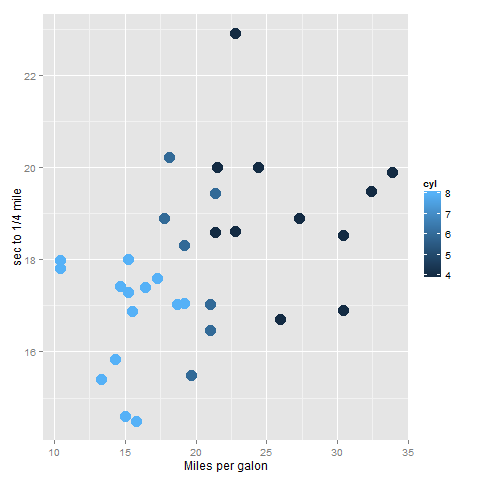
\includegraphics[width=10cm]{fig/plot1} % not necessary to give extension - now you can shift between compiling to ps or to pdf without any problems
 
\caption[Do not end short caption with full-stop]{Each figure must be supplied with a long caption, making the figure stand-alone and ended with a full-stop.}

\end{figure}





\newpage





% SUBFIG EXAMPLE
%================
%
% usage: \subfloat[][caption]{...figure code...\label{label}}

The subfigures are Figures \subref{firstfigure}, \subref{secondfigure}, \subref{thirdfigure} and \subref{fourthfigure}.

\begin{figure}
\centering

\subfloat[][First subcaption (No full-stop)]{
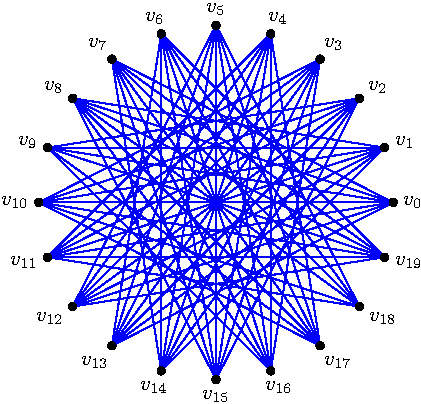
\includegraphics{fig/figure}
\label{firstfigure}
}
\quad
\subfloat[][Second subcaption (No full-stop)]{
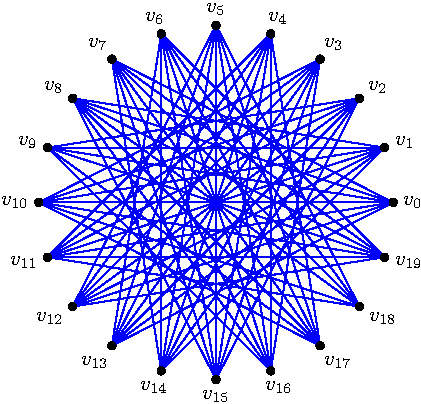
\includegraphics{fig/figure}
\label{secondfigure}
}
\\
\subfloat[][Third subcaption (No full-stop)]{
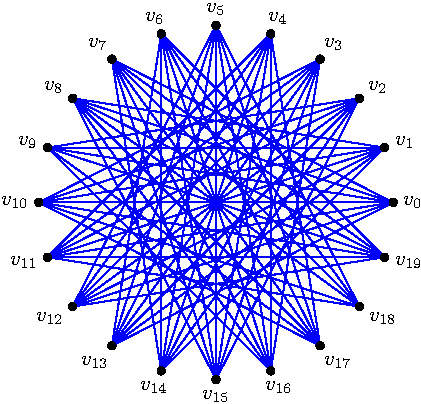
\includegraphics{fig/figure}
\label{thirdfigure}
}
\quad
\subfloat[][Fourth subcaption (No full-stop)]{
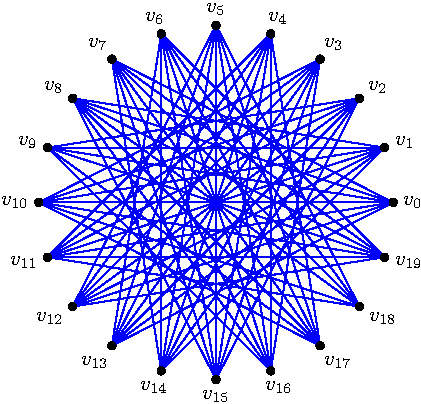
\includegraphics{fig/figure}
\label{fourthfigure}
}
\caption[Do not end short caption with full-stop]{End the main caption with a full-stop, but not each of the sub-figure captions!}
\label{thislabel}
\end{figure}
            % remove if NA
%%%%%%%%%%%%%%%%%%%%%%%%%%%%%%%%%%%%%%%%%%%%%%%%
%
% how to typeset algorithms
%
%%%%%%%%%%%%%%%%%%%%%%%%%%%%%%%%%%%%%%%%%%%%%%%%
\chapter{Algorithms}

% USE THE TEMPLATE BELOW FOR YOUR ALGORITHMS
%============================================
%
% \begin{algorithm}
% 
% \SetKwInOut{Input}{Input}
% \SetKwInOut{Output}{Output}
% 
% \Indm
% \Input{Description of the input to the algorithm.}
% \Output{Description of the output from the algorithm.}
% \Indp
% 
% \BlankLine
% 
%   % main algorithm code here
% 
% \caption{Algorithm example}
% \label{alg}
%
% \end{algorithm}



\begin{algorithm}

\SetKwInOut{Input}{Input}
\SetKwInOut{Output}{Output}

\SetKwData{Left}{left}
\SetKwData{This}{this}
\SetKwData{Up}{up}
\SetKwFunction{Union}{Union}
\SetKwFunction{FindCompress}{FindCompress}

\Indm
\Input{Description of the input to the algorithm.}
\Output{Description of the output from the algorithm.}
\Indp

\BlankLine

\emph{special treatment of the first line}\;
\For{$i\leftarrow 2$ \KwTo $l$}{
  \emph{special treatment of the first element of line $i$}\;
  \For{$j\leftarrow 2$ \KwTo $w$}{\label{forins}
    \Left$\leftarrow$ \FindCompress{$Im[i,j-1]$}\;
    \Up$\leftarrow$ \FindCompress{$Im[i-1,]$}\;
    \This$\leftarrow$ \FindCompress{$Im[i,j]$}\;
    \If{\Left compatible with \This}{\label{lt}
      \lIf{\Left $<$ \This}{\Union{\Left,\This}}\;
      \lElse{\Union{\This,\Left}\;}
    }
    \If{\Up compatible with \This}{\label{ut}
      \lIf{\Up $<$ \This}{\Union{\Up,\This}}\;
      \lElse{\Union{\This,\Up}}
    }
  }
  \lForEach{element $e$ of the line $i$}{\FindCompress{p}}
}

\caption[Do not end short caption with full-stop]{Algorithm example}
\label{alg}

\end{algorithm}




\begin{algorithm}[t]
%\SetAlgoNoLine
 \Input{A tree $T$ represented by an array {\sf Parent}$[1,\ldots,n]$.}
\Output{A minimum secure dominating set of $T$, represented by a boolean array $X$.}
\For{$i\leftarrow 1$ to $n$}{
{\sf A3Label}$[i] \leftarrow$ {\sc False}\;
$X[i] \leftarrow$ {\sc False}\;
{\sf Labels}$[i] \leftarrow [0,0,0,0,0,0,0]$\;
{\bf if} vertex $i$ is a anchor of $T$ {\bf then} {\sf Branch}$[i] \leftarrow$ {\sc True}\;
{\sf Previous1Label}$[i] \leftarrow 0$\;
}
\For{$i\leftarrow n$ down to $2$}{
$\ell \leftarrow$ {\sf\bf EffectiveLabel}({\sf Labels}[$i$])\;
{\bf if} $\ell$ is odd {\bf then} $X[i] \leftarrow ${\sc True}\;
{\sf Labels$[$Parent$[i],\ell(i)+1 \ (\rm{mod}\ 7)]$} $++$\;
\If{$\ell=2$ {\bf and} {\sf Branch$[$Parent$[i]]$}}{
{\sf A3Label[Parent}$[i]] \leftarrow$ {\sc True}\;
{\sf prev} $\leftarrow$ {\sf Previous1Label$[$Parent$[i]]$}\;
{\bf if} {\sf prev} $>0$ {\bf then} $X[${\sf prev}$] \leftarrow$ {\sc True}\;
}
\If{$\ell=0$ {\bf and} {\sf Branch$[$Parent$[i]]$}}{
\If{{\sf A3Label$[$Parent$[i]]$}}{
$X[i] \leftarrow$ {\sc True}\;
}
\Else{
{\sf prev} $\leftarrow$ {\sf Previous1Label$[$Parent$[i]]$}\;
{\bf if} {\sf prev} $>0$ {\bf then} $X[${\sf prev}$] \leftarrow$ {\sc True}\;
{\sf Previous1Label$[$Parent$[i]] \leftarrow i$}\;
}
}
}
$\ell \leftarrow$ {\sf\bf EffectiveLabel}({\sf Labels}[$1$])\;
{\bf if} $\ell$ is odd {\bf then} $X[1] \leftarrow ${\sc True}\;
{\bf if}  {\sf Labels}$[1,j]=0$ for $j=1,3,4,5,6$ {\bf then} $X[1] \leftarrow$ {\sc True}\;
{\bf if} {\sf Labels}$[1,j]=0$ for $j=1,3,5,6$ {\bf and} {\sf Labels}$[1,0] \geq |${\sf Labels}$[1]-1|$  {\bf then} $X[1] \leftarrow$ {\sc True}\;
\If{$\ell=3$}{
{\sf prev} $\leftarrow$ {\sf Previous1Label$[1]$}\;
{\bf if} {\sf prev} $ > 0$ {\bf then} $X[$\sf{prev}$]$ $\leftarrow$ {\sc True}\;
}
\Return[$X$]\;
\caption[{{Do not end short caption with full-stop}}]{{\sf\bf DefendTree}}
\label{Alg:Tree}
\end{algorithm}

         % remove if NA


%=================================================
% include your chapters here
%=================================================
%%%%%%%%%%%%%%%%%%%%%%%%%%%%%%%%%%%%%%%%%%%%%%%%
%
% start writing
%
%%%%%%%%%%%%%%%%%%%%%%%%%%%%%%%%%%%%%%%%%%%%%%%%


\chapter{Introduction}
% put these two lines after every \chapter{} command
\vspace{-2em}
\minitoc

\startarabicpagenumbering % must be just after the first \chapter{} command


\blindtext

\section{Background}

\blindtext

\blindtext

\section{Informal problem description}

\blindtext

\blindtext

\section{Research hypothesis}

\Blindtext

\section{Scope and objectives}

The following objectives will be pursued in this project/thesis/dissertation:
\begin{enumerate}[label=\Roman*]										% \usepackage{enumitem}
 \item To \textit{conduct} a thorough survey of the literature related to:
 \begin{enumerate}[label=(\alph*)]
  \item facility location problems in general,
  \item models for the placement of a network of radio transmitters in particular,
  \item the nature of parameters required to describe effective radio transmission, and
  \item terrain elevation data required to generate an instance of the bi-objective radio transmitter location problem described in the previous section.
 \end{enumerate}
 \item  To \textit{establish} an suitable framework for evaluating the effectiveness of a given set of placement locations for a network of radio transmitters in respect of its total area coverage and its mutual area coverage.
 \item To \textit{formulate} a bi-objective facility location model suitable as a basis for decision support in respect of the location of a network of radio transmitters with a view to identify high-quality trade-offs between maximising total coverage area and maximising mutual coverage area.  The model should take as input the parameters and data identified in Objective~I(c)--(d) and function within the context of the framework of Objective~II.
 \item To \textit{design} a generic \textit{decision support system} (DSS) capable of suggesting high-quality trade-off locations for user-specified instances of the bi-objective radio transmitter location problem described in the previous section.  This DSS should incorporate the location model of Objective~III.
 \item To \textit{implement} a concept demonstrator of the DSS of Objective IV in an applicable software platform.  This DSS should be flexible in the sense of being able to take as input an instance of the bi-objective radio transmitter location problem described in the previous section via user-specification of the parameters and data of Objectives I(c)--(d) and produce as output a set of high-quality trade-off transmitter locations for that instance.
 \item To \textit{verify} and validate the implementation of Objective V according to generally accepted modelling guidelines.
 \item To \textit{apply} the concept demonstrator of Objective V to a special case study involving realistic radio transmission parameters and real elevation data for a specified portion of terrain.
 \item To \textit{evaluate} the effectiveness of the DSS and associated concept demonstrator of Objectives~IV--VI in terms of its capability to identify a set of high-quality trade-off solutions for a network of radio transmitter locations.
 \item To \textit{recommend} sensible follow-up work related to the work in this project which may be pursued in future.
\end{enumerate}

\section{Research methodology}
\blindtext

\section{Project/thesis/dissertation organisation}
\blindtext
%%%%%%%%%%%%%%%%%%%%%%%%%%%%%%%%%%%%%%%%%%%%%%%%
%
% start writing
%
%%%%%%%%%%%%%%%%%%%%%%%%%%%%%%%%%%%%%%%%%%%%%%%%


\chapter{Conclusion}
% put these two lines after every \chapter{} command
\vspace{-2em}
\minitoc

%\startarabicpagenumbering % must be just after the first \chapter{} command


\blindtext

\section{Project/thesis/dissertation summary}

\blindtext

\blindtext

\section{Appraisal of project/thesis/dissertation contributions}

\blindtext

\section{Suggestions for future work}

\blindtext

\section{What the student has learnt during this project}		%ONly for skripsie students

\blindtext


%=================================================
% bibliography
%=================================================
\cite{*} % cites all items in your .bib file for the purpose of testing biblatex - REMOVE!
\printbibliography[heading=bibintoc] % prints a bibliography containing all (and only) cited items


%=================================================
% Appendices
%=================================================
\appendix
\chapter{Project Timeline}

The expected timeline is given in Figure \ref{Ganttchart} in Gantt-chart form.


\begin{figure}[htb]
\centering
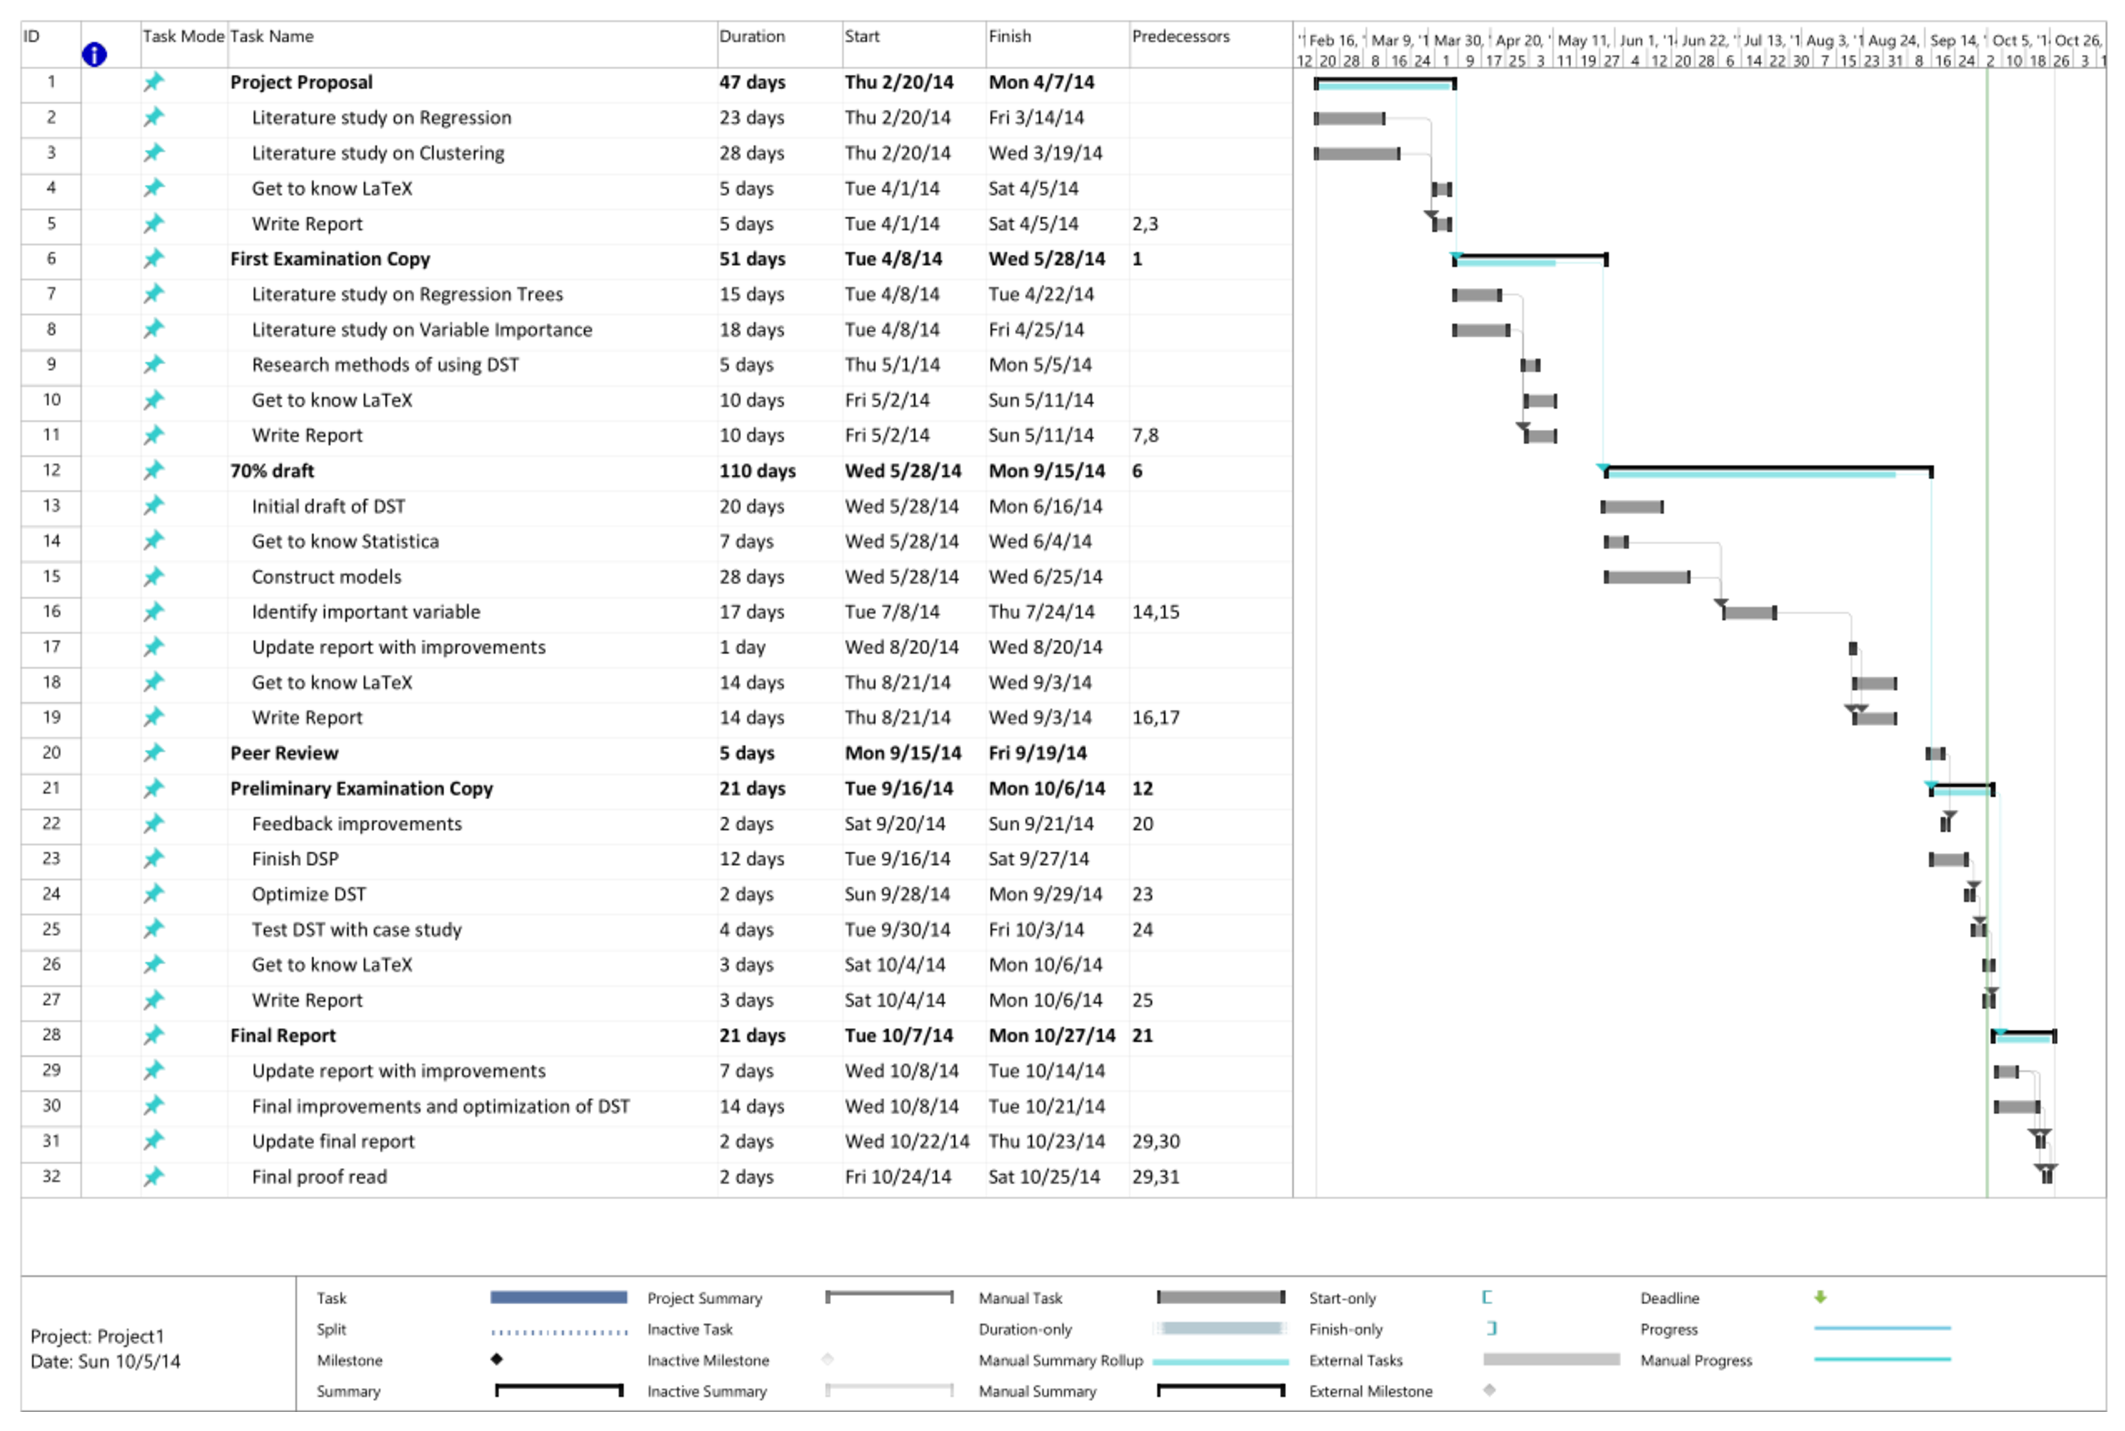
\includegraphics[angle=90,scale=0.6,trim=0 0 0 0, clip]{examples/Timeline}
%\leftskip-1.5cm
\caption{Expected timeline in Gannt-chart form.}
\label{Ganttchart}
\end{figure}
\chapter{Data}

% EXAMPLE
%=========
%
% example using multicolumn, multirow and the sideways environment
Data related to the Case Study in Chapter 5 are presented in Table \ref{ex2}.
\begin{table}[h!tb]

\centering

\begin{tabular}{cc|rrrrrr}\hline

\headcol &&\multicolumn{6}{c}{this goes across 6 columns}\\

 \headcol && col a & col b & col c & col d & col e & col f \\ \hline \hline

\multirow{6}{*}{
%
\begin{sideways}
this is sideways,
\end{sideways}
%
\begin{sideways}
and goes across
\end{sideways}
%
\begin{sideways}
six rows
\end{sideways}
%
}


& row 1 \\
& row 2 & \cellcolrow & \cellcolrow & \cellcolrow & \cellcolrow & \cellcolrow & \cellcolrow \\
& row 3 \\ 
& row 4 & \cellcolrow & \cellcolrow & \cellcolrow & \cellcolrow & \cellcolrow & \cellcolrow \\
& row 5 \\
& row 6 & \cellcolrow & \cellcolrow & \cellcolrow & \cellcolrow & \cellcolrow & \cellcolrow \\ \hline

\end{tabular}

\caption[Do not end short caption with full-stop]{Type full caption here.}
\label{ex2}

\end{table}



\end{document}
